% Research Background Chapter
\subsection{Background and Motivation}


Until recently, radar technology was primarily associated with high-end vehicles and military applications. However, today, the same technology is being used in everyday objects such as table lamps and smart speakers.

For instance, the \cite{Aqara_Presence_Sensor_FP2} home presence sensor is capable of detecting up to five individuals and responding to their movements, all while remaining unobtrusive and serving as an alternative to traditional surveillance methods.



The development and production of mobile robots is currently a rapidly growing field. Such robots are used both in the industrial sector and in everyday life. Research and development of mobile robots is being actively carried out to eliminate the consequences of natural and man-made disasters, for the needs of the military-industrial complex and space research. In this regard, the creation of mobile robots is not only a commercially profitable and scientifically significant direction, but also a strategically important task for the state and society as a whole.  

The history of their evolution reflects the achievements in the field of robotics. The list summarises the key milestones in the speed increase of mobile robots and the specifics of their applications. The increasing speed of mobile robots inevitably leads to increasing demands on their internal systems. This applies both to the power of actuators, the accuracy of sensor systems, and control algorithms\citep{turn0search0}.


Traditionally, robotic systems have relied on light sensors such as cameras and lidars to build a view of the environment. Unfortunately, cameras and lidars are not universally functional when faced with illuminated or structurally degraded cases. Despite consistent developments on photometric calibration\citep{PointLightYang}, camera distortion calibration \citep{Jin2019} 

\begin{figure}[H]
    \centering
    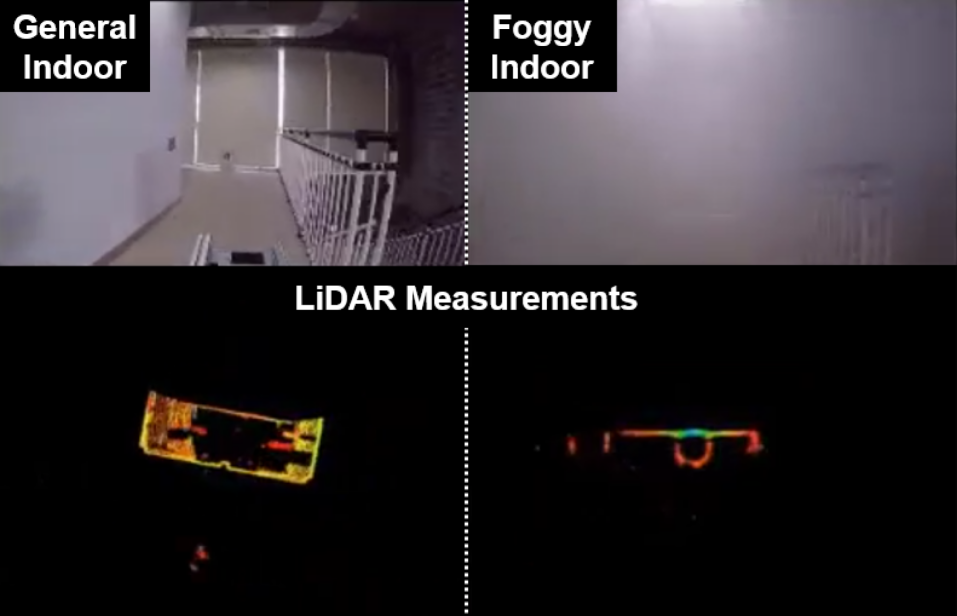
\includegraphics[width=\linewidth]{Src/images/x1.png} 
    \caption{Lidar measurements in a foggy indoor environment \citep{harlow2021mmwave}}
    \label{fig:lidarfogy}
\end{figure}
 
Navigational situations that seriously impair the camera \citep{starr2013navigation} and lidar \citep{radio1943detection} as seen on figure 1 but not the radar include smoke, dust, fog, rain, and snow. Radars can theoretically pass through the different types of tiny particulate matter by using longer wavelengths. 

Radar technology, although widely used in meteorology, target tracking, planetary mapping, and automotive safety, remains underutilized in robotics compared to shorter wavelength sensors like cameras and lidars. Radar systems transmit and receive specially shaped electromagnetic pulses to determine the distance and direction of objects, offering advanced sensing capabilities. This makes radar a valuable option for integration with existing systems or as an independent sensor, enabling robots to perform both metric and semantic tasks reliably.

The advent of mWave radars operating in the 76–81 GHz range provides a compact and alternative to lidar . 

\begin{figure}[H]
    \centering
    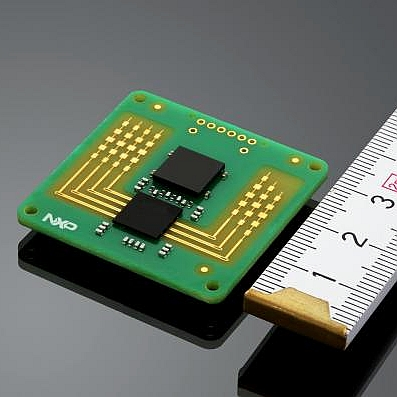
\includegraphics[width=\linewidth/2]{Src/images/automotive-radars.jpg} 
    \caption{Radar sensors \citep{tusur_radar_sensors}}
    \label{fig:radarsensor}
\end{figure}
In recent years, there has been a significant increase in the number of devices utilizing millimeter-wave (mmWave) radars. Most existing solutions are represented by radar-on-chip systems. A radar-on-chip is an integrated system that combines radar functionality into a single compact microchip device (Figure 1.2), making it applicable in various fields. Recent developments are focused on replacing presence sensors (PIR), with the primary goal being the detection of humans.\citep{s24113660}.

However, there are some reasons why robotics does not frequently use millimeter wave radars. Radar has numerous issues that need to be taken into account while creating new solutions, just like any other sensor. False reflections beyond the sensor's range, more intricate speckle noise, and multipath reflections—which produce several reflections from a single object—are just a few of the distinctive noise features of radar. 

Clustering-based filtering algorithms, such CFAR \citep{finn1968adaptive}, OPTICS \citep{nitzberg1972cfar}, and DBSCAN \citep{ankerst1999optics}, assist in reducing unwanted reflections and speckle noise, although require to be carefully tuned to fit particular hardware and antenna radiation patterns. Enhancing radar sensors themselves with greater resolution and quicker scanning rates can help with this to some extent. However, using various map formats, features, and internal state estimators also allows for algorithmic improvements.

The use of radar sensors in autonomous robots is an optimal solution because a robot is typically a complex collection of different systems. With other sensors, such as inertial sensors or odometers, the robot can determine its current speed, making it much easier to integrate and work with new types of sensors, including radar sensors. This allows for more reliable and accurate perception of the environment.


\subsection{Problem Statement}


\subsection{ Research Aim and Objectives}
The aim of the work is to develop the principles of construction, as well as the algorithmic and software of the information radar system of a mobile robot.


%%%%%%%%%%%%%%%%%%%%%%%%%%%%%%%%%%%%%%%%%%%%%%%%%%%%%%%%%%%%%%%%%%%%%%%%%%%%%%%%%%%%%%
\paragraph{Research Objectives}
An information system for detecting and tracking fast-moving objects in robotics applications.


%%%%%%%%%%%%%%%%%%%%%%%%%%%%%%%%%%%%%%%%%%%%%%%%%%%%%%%%%%%%%%%%%%%%%%%%%%%%%%%%%%%%%%
\paragraph{Research Subject}
Mathematical models of navigation processes for the detection of selected dynamic objects using FMCW radar systems.




%%%%%%%%%%%%%%%%%%%%%%%%%%%%%%%%%%%%%%%%%%%%%%%%%%%%%%%%%%%%%%%%%%%%%%%%%%%%%%%%%%%%%%
\subsection{Research Questions and Hypotheses}







%%%%%%%%%%%%%%%%%%%%%%%%%%%%%%%%%%%%%%%%%%%%%%%%%%%%%%%%%%%%%%%%%%%%%%%%%%%%%%%%%%%%%%
\subsection{Tasks}



%%%%%%%%%%%%%%%%%%%%%%%%%%%%%%%%%%%%%%%%%%%%%%%%%%%%%%%%%%%%%%%%%%%%%%%%%%%%%%%%%%%%%%
\subsection{Scope and Delimitations}



%%%%%%%%%%%%%%%%%%%%%%%%%%%%%%%%%%%%%%%%%%%%%%%%%%%%%%%%%%%%%%%%%%%%%%%%%%%%%%%%%%%%%%


